\chapter{J-Horror: Ringu, Ju-on and the Modern Onryō}

\section{What is J-horror?}

\begin{definition}[J-horror]
\emph{J-horror} (\ja{ジャパニーズホラー}) is the wave of Japanese horror films, many
low-budget and first released on video, that began in the 1990s, peaked with
\emph{Ringu} (1998) and \emph{Ju-on} (2002), and was remade by Hollywood in the 2000s. Its
signature figure is the long-haired female ghost, a modern \emph{onryō}.
\end{definition}

\subsection{Characteristics}

\begin{itemize}
  \item \textbf{Slow dread rather than shock}: long takes, ambient sound, little music,
        things glimpsed at the edge of the frame. Violence is often off-screen.
  \item \textbf{Ordinary settings}: apartments, schools, offices, suburban houses, rather
        than castles or haunted mansions.
  \item \textbf{Technology as medium}: videotapes, phones, televisions, the internet
        (\emph{Kairo}, 2001) carry the curse.
  \item \textbf{Curses that spread}: the ghost's rage is not limited to those who wronged
        her; it spreads virally to anyone who comes into contact with it. There is no
        resolution through justice.
  \item \textbf{The family}: absent fathers, isolated mothers, abused or abandoned children.
\end{itemize}

\section{Genealogy of the female ghost}

\begin{center}
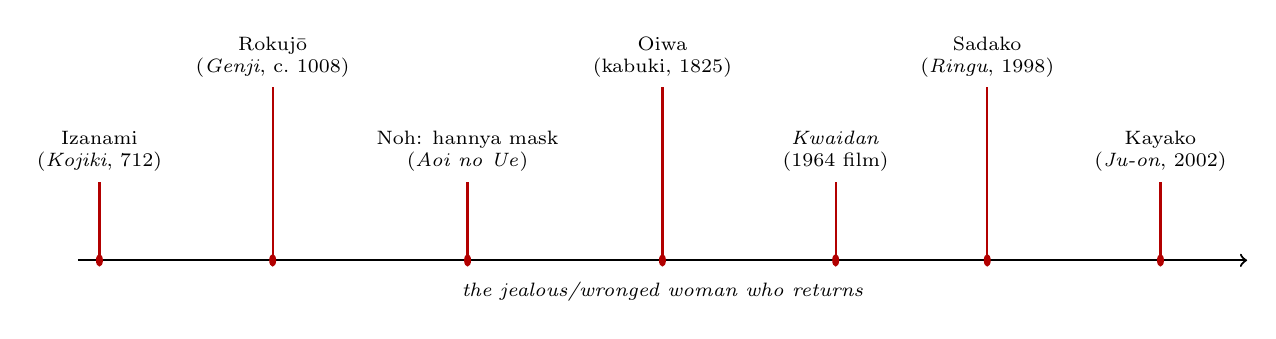
\begin{tikzpicture}[x=0.55cm, y=1cm, every node/.style={font=\scriptsize}]
  \draw[->, thick] (0,0) -- (27,0);
  \foreach \x/\h/\lab in {0.5/1.0/{Izanami\\(\emph{Kojiki}, 712)}, 4.5/2.2/{Rokujō\\(\emph{Genji}, c.\ 1008)},
      9/1.0/{Noh: hannya mask\\(\emph{Aoi no Ue})}, 13.5/2.2/{Oiwa\\(kabuki, 1825)}, 17.5/1.0/{\emph{Kwaidan}\\(1964 film)},
      21/2.2/{Sadako\\(\emph{Ringu}, 1998)}, 25/1.0/{Kayako\\(\emph{Ju-on}, 2002)}} {
    \draw[red!70!black, thick] (\x,0) -- (\x,\h);
    \node[above, align=center] at (\x,\h) {\lab};
    \fill[red!70!black] (\x,0) circle (0.08);
  }
  \node[below, font=\scriptsize\itshape] at (13.5,-0.15) {the jealous/wronged woman who returns};
\end{tikzpicture}
\end{center}

\section{\emph{Ringu} (1998)}

\begin{center}
\begin{tabular}{ll}
\toprule
Source & Suzuki Kōji's novel \emph{Ringu} (\ja{リング}, 1991) \\
Director & Nakata Hideo \\
Screenplay & Takahashi Hiroshi \\
Remake & \emph{The Ring} (Gore Verbinski, 2002) \\
\bottomrule
\end{tabular}
\end{center}

\subsection{Plot}

\begin{enumerate}
  \item An urban legend circulates among teenagers: watch a certain videotape and you will
        receive a phone call and die in exactly \textbf{seven days}. A schoolgirl dies with a
        face frozen in terror.
  \item Her aunt, the TV journalist \textbf{Asakawa Reiko}, investigates, finds the tape
        at a resort cabin on the Izu peninsula, watches it, and gets the phone call. Her
        ex-husband Ryūji (a psychic academic) and their young son Yōichi also see the tape.
  \item The tape's images lead them to \textbf{Yamamura Shizuko}, a psychic woman from
        Ōshima island publicly humiliated in a demonstration before journalists in the
        1950s (modelled on the Meiji psychic experiments, Week 7), and her daughter
        \textbf{Sadako} (\ja{貞子}), who had terrifying powers.
  \item They discover that Sadako was thrown into a well by Dr.\ Ikuma, Shizuko's lover and probably Sadako's father, and left
        to die. They find her remains under the cabin and Reiko embraces her skull. Reiko
        survives the seventh day and thinks the curse is lifted.
  \item But Ryūji dies: Sadako crawls out of a well on his television screen and out of the
        TV into his room. Reiko realizes she survived because she \emph{copied the tape and
        showed it to someone else}. To save her son, she drives to her father's house with
        the tape.
\end{enumerate}

\begin{important}[Reading Sadako]
\begin{itemize}
  \item \textbf{Iconography}: white dress, long black hair over the face, contorted
        movements (the actor was filmed walking backwards and the film reversed): Oiwa and
        the Edo yūrei updated.
  \item \textbf{The well}: wells are traditional sites of ghosts (the \emph{Banchō
        Sarayashiki} ghost Okiku counts plates from a well). Sadako's well links new
        technology to old folklore.
  \item \textbf{The curse as virus/media}: the tape must be copied and passed on, like a
        chain letter or a computer virus. Horror is about media circulation itself.
  \item \textbf{Unredeemable rage}: unlike Michizane, Sadako cannot be pacified. Finding
        her body (a proper burial, the classic solution) does not work. Some critics link
        this to 1990s anxieties: the burst bubble, the 1995 Kobe earthquake and the Aum
        Shinrikyō subway gas attack, a sense that institutions could no longer protect.
  \item \textbf{Motherhood}: Reiko is a working single mother; the film's horror often
        centres on mothers and children.
\end{itemize}
\end{important}

\section{\emph{Ju-on} (2002)}

\begin{center}
\begin{tabular}{ll}
\toprule
Director & Shimizu Takashi \\
Versions & V-cinema videos (2000), theatrical film (2002), US remake \emph{The Grudge} (2004, also by Shimizu) \\
Ghosts & Kayako (\ja{伽椰子}) and her son Toshio \\
\bottomrule
\end{tabular}
\end{center}

\begin{definition}[Ju-on]
\emph{Ju-on} (\ja{呪怨}, ``curse-grudge''): the film's opening title explains that when a
person dies in the grip of a powerful rage, a curse is born that gathers in the place of
death; anyone who encounters it is consumed by it, and the curse is renewed.
\end{definition}

\begin{itemize}
  \item A housewife, Kayako, is murdered by her jealous husband, who also kills their son
        Toshio and the family cat. Their house in a Tokyo suburb becomes cursed.
  \item The film is told in non-chronological segments named after victims: a social
        worker, a family who moves in, a schoolgirl, police officers. Each enters the
        house and is taken.
  \item Kayako's signature: a death rattle (\emph{a croaking sound} made in her throat),
        crawling down stairs with broken limbs; Toshio's pale face and cat-like cry.
\end{itemize}

\begin{remark}
\emph{Ju-on} reverses the classic onryō logic: the curse attaches to a \emph{place}
(like a yōkai in Yanagita's distinction) and attacks people who never wronged Kayako. The
ghost is no longer a moral agent seeking justice but a contagion. The house is an ordinary
two-storey suburban home, the dream of the postwar middle class turned into a trap.
\end{remark}

\section{Comparing Oiwa, Sadako and Kayako}

\begin{center}
\begin{tabular}{p{2.8cm}p{3.4cm}p{3.4cm}p{3.4cm}}
\toprule
 & Oiwa (1825) & Sadako (1998) & Kayako (2002) \\
\midrule
Wronged by & husband (betrayal, poison) & father figure (thrown in a well) & husband (jealous murder) \\
Targets & the guilty (Iemon and accomplices) & anyone who watches the tape & anyone who enters the house \\
Medium & stage tricks & videotape, TV & house, photographs \\
Escape & none for the guilty & copy the tape (pass it on) & none \\
Body & disfigured face, falling hair & hidden face, long hair & broken body, croak \\
\bottomrule
\end{tabular}
\end{center}

\section{The Hollywood remake boom}

\begin{itemize}
  \item \emph{The Ring} (2002) earned far more worldwide than the original; this led to
        remakes of \emph{Ju-on} (\emph{The Grudge}, 2004), \emph{Dark Water} (2005),
        \emph{One Missed Call} (2008) and \emph{Pulse} (2006, from \emph{Kairo}).
  \item The remakes generally added backstory and explanation, Christian or psychological
        frames, and louder jump scares; critics thought they lost the ambiguity of the
        originals.
  \item J-horror influenced Korean horror (\emph{A Tale of Two Sisters}, 2003) and the
        broader ``Asian Extreme'' marketing category in the West.
  \item The long-haired ghost became a global meme, parodied and eventually cute: Sadako
        threw the first pitch at a baseball game in 2012, and \emph{Sadako vs.\ Kayako}
        (2016) treated the two ghosts as a franchise crossover, like Godzilla vs.\ King
        Kong.
\end{itemize}

\begin{aside}
In tutorial we argued about whether J-horror is ``traditional''. My group's answer: the
\emph{imagery} is traditional (Edo yūrei, the well, the grudge), but the \emph{logic} is
modern (anonymous media, viral spread, no pacification). Sadako is what an onryō looks
like when there is no longer a community to enshrine her.
\end{aside}

\section*{Summary}
\begin{itemize}
  \item J-horror (1990s--2000s): slow dread, everyday settings, technology as medium,
        long-haired female ghosts.
  \item \emph{Ringu} (Nakata, 1998): Sadako's cursed videotape; survival only by passing
        the curse on.
  \item \emph{Ju-on} (Shimizu, 2002): Kayako's curse attaches to a house and spreads to
        anyone who enters.
  \item Modern onryō cannot be pacified: rage becomes contagion.
  \item Hollywood remakes globalized the imagery and eventually turned it into parody and
        merchandise.
\end{itemize}
